\documentclass[letterpaper,14pt,titlepage,fleqn]{article}

\setlength{\mathindent}{1cm}

\usepackage{graphicx}                                        

\usepackage{amssymb}                                         
\usepackage{amsmath}                                         
\usepackage{amsthm}                                          

\usepackage{alltt}                                           
\usepackage{float}
\usepackage{color}

\usepackage{url}

\usepackage{balance}
\usepackage[TABBOTCAP, tight]{subfigure}
\usepackage{enumitem}

\usepackage{pstricks, pst-node}

\usepackage{cite}
\usepackage{indentfirst}
\usepackage{listings}

% the following sets the geometry of the page
\usepackage{geometry}
\geometry{textheight=9in, textwidth=6.5in}

% random comment

\newcommand{\cred}[1]{{\color{red}#1}}
\newcommand{\cblue}[1]{{\color{blue}#1}}

\usepackage{hyperref}

\usepackage{textcomp}
\usepackage{listings}

\def\name{Haoxiang Wang; Student ID: 932359049}

%% The following metadata will show up in the PDF properties
\hypersetup{
  colorlinks = true,
  urlcolor = black,
  pdfauthor = {\name},
  pdfkeywords = {CS557 Project 4},
  pdftitle = {Project \#4: Displacement Mapping, Lighting, and Bump Mapping},
  pdfsubject = {Project \#4: Displacement Mapping, Lighting, and Bump Mapping},
  pdfpagemode = UseNone
}

\parindent = 0.0 in
\parskip = 0.2 in

\author{\name}
\title{Project \#4: Displacement Mapping, Lighting, and Bump Mapping}

\begin{document}
\maketitle

This project is the fourth project I have done in this class, and it is the second project that working with GLSL. Since we gained the experience of \textit{GLman} and \textit{GLSL} from last project, this project seems easy to deal with, and the result turned out that the most part of the project was as easy as I expected except one problem I spent days to fix. The main part of the project takes me around half a day to get everything done and fit to all the requirements, and the problem takes me two days to fix it. The source listing, the results images and the explanation of how code works will be described in the after section. 

\section{Source Listing}
In this project, three files are necessary. They are .glib file, .vert file, and .frag file. No .obj file is needed in this project. The specific filenames and usages are listed below.

coscos.glib --- Handle the user interface and object

coscos.vert --- Handle the vertex shader

coscos.frag --- handle the fragment shader

\section{Result Images and Explanation}
The requirements of this project can be simply divided into two parts. The first one is to put the real displacement on a flat plane in order to create a $cos*cos$ pattern. The second part is to implement the bump mapping with noise on the displaced surface. We also need to implement the fragment lighting to deliver the sense that our displacement and the bump mapping is correct. We have already done something with displacement and bump mapping with \textit{RenderMan} in project 2, when implementing them again with GLSL, the situation differs, the biggest difference will be introduced in the following section. The following image shows that original image and the variable values when the image is rendered. 
\begin{center}
	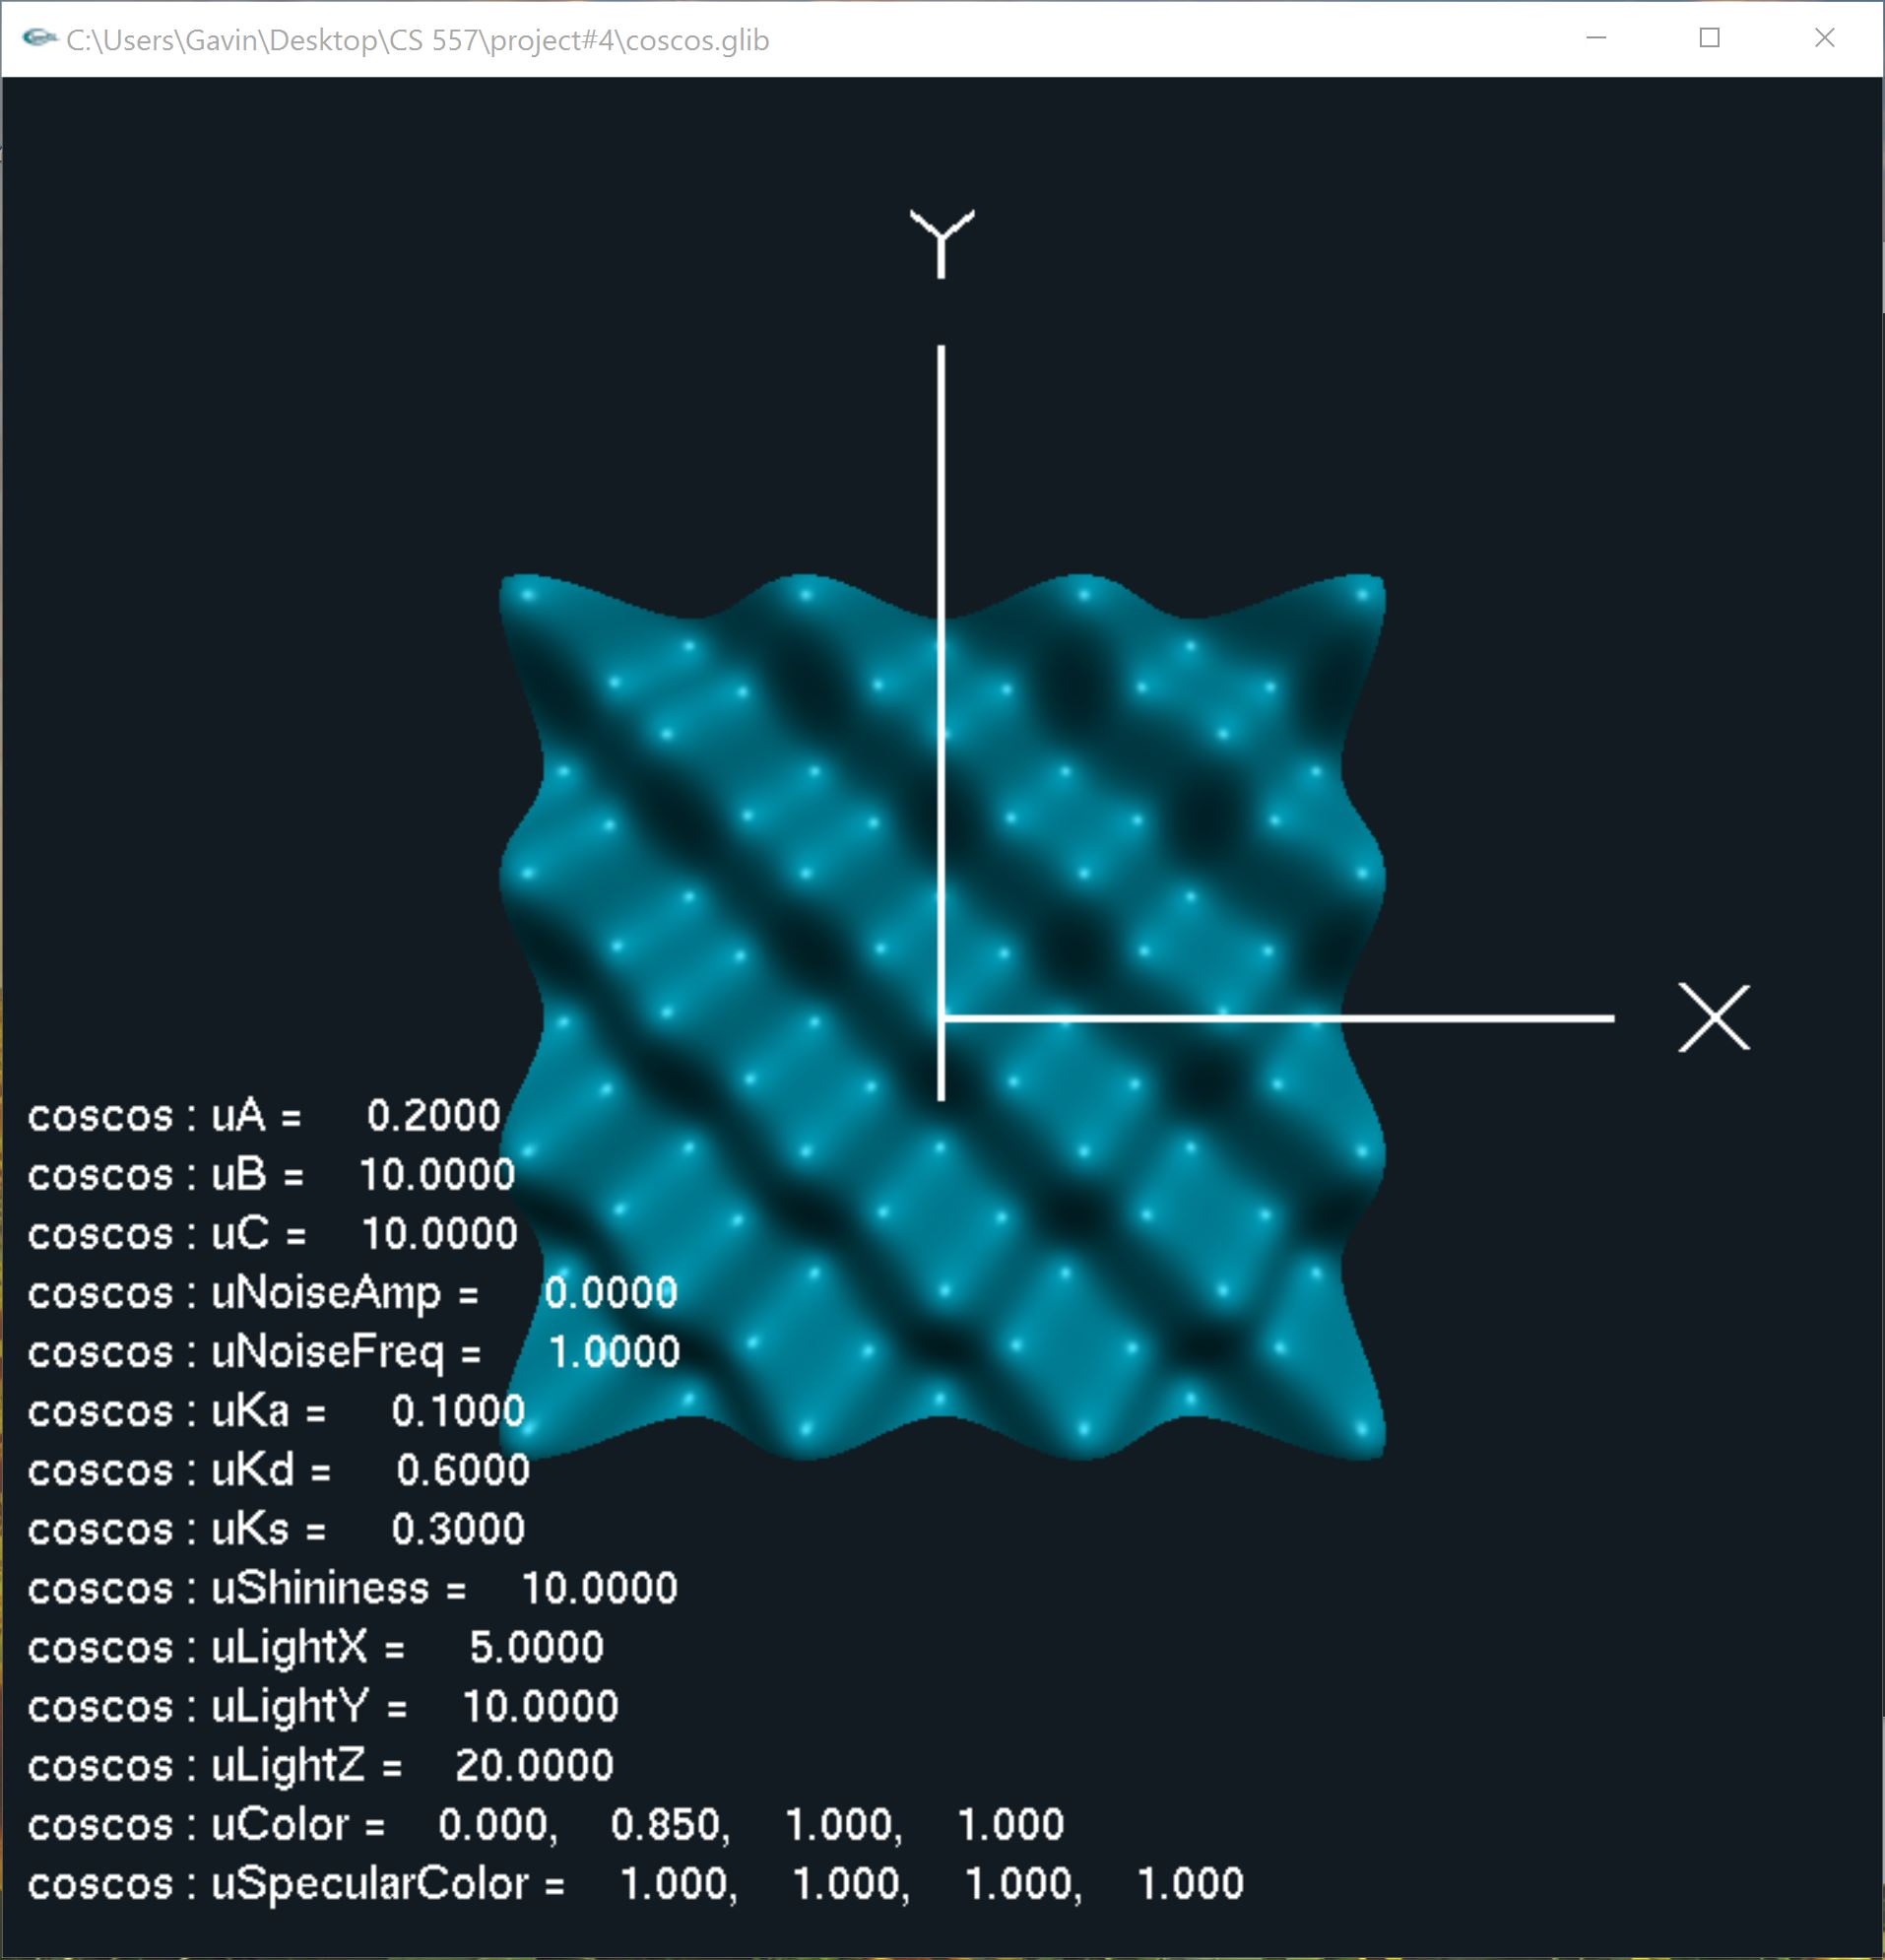
\includegraphics[width=3in]{origin.jpg}
\end{center}
The original image shows the eye looking at the plane through a vertical direction, which makes the lighting looks not really straightforward. By rotating the whole plane with an angle, the correctness of fragment lighting could be examined. The biggest difference between this project and the project 2 is that GLSL doesn't have the  normal calculate function like RenderMan does. In order to implement the correct lighting, we need to calculate the normal manually in the code. The way is to take two tangent value from x and y direction, and them apply a cross product on them. By doing this with every fragment, the correct normal will be produced. The following image shows the fragment lighting I have in in the project.
\begin{center}
	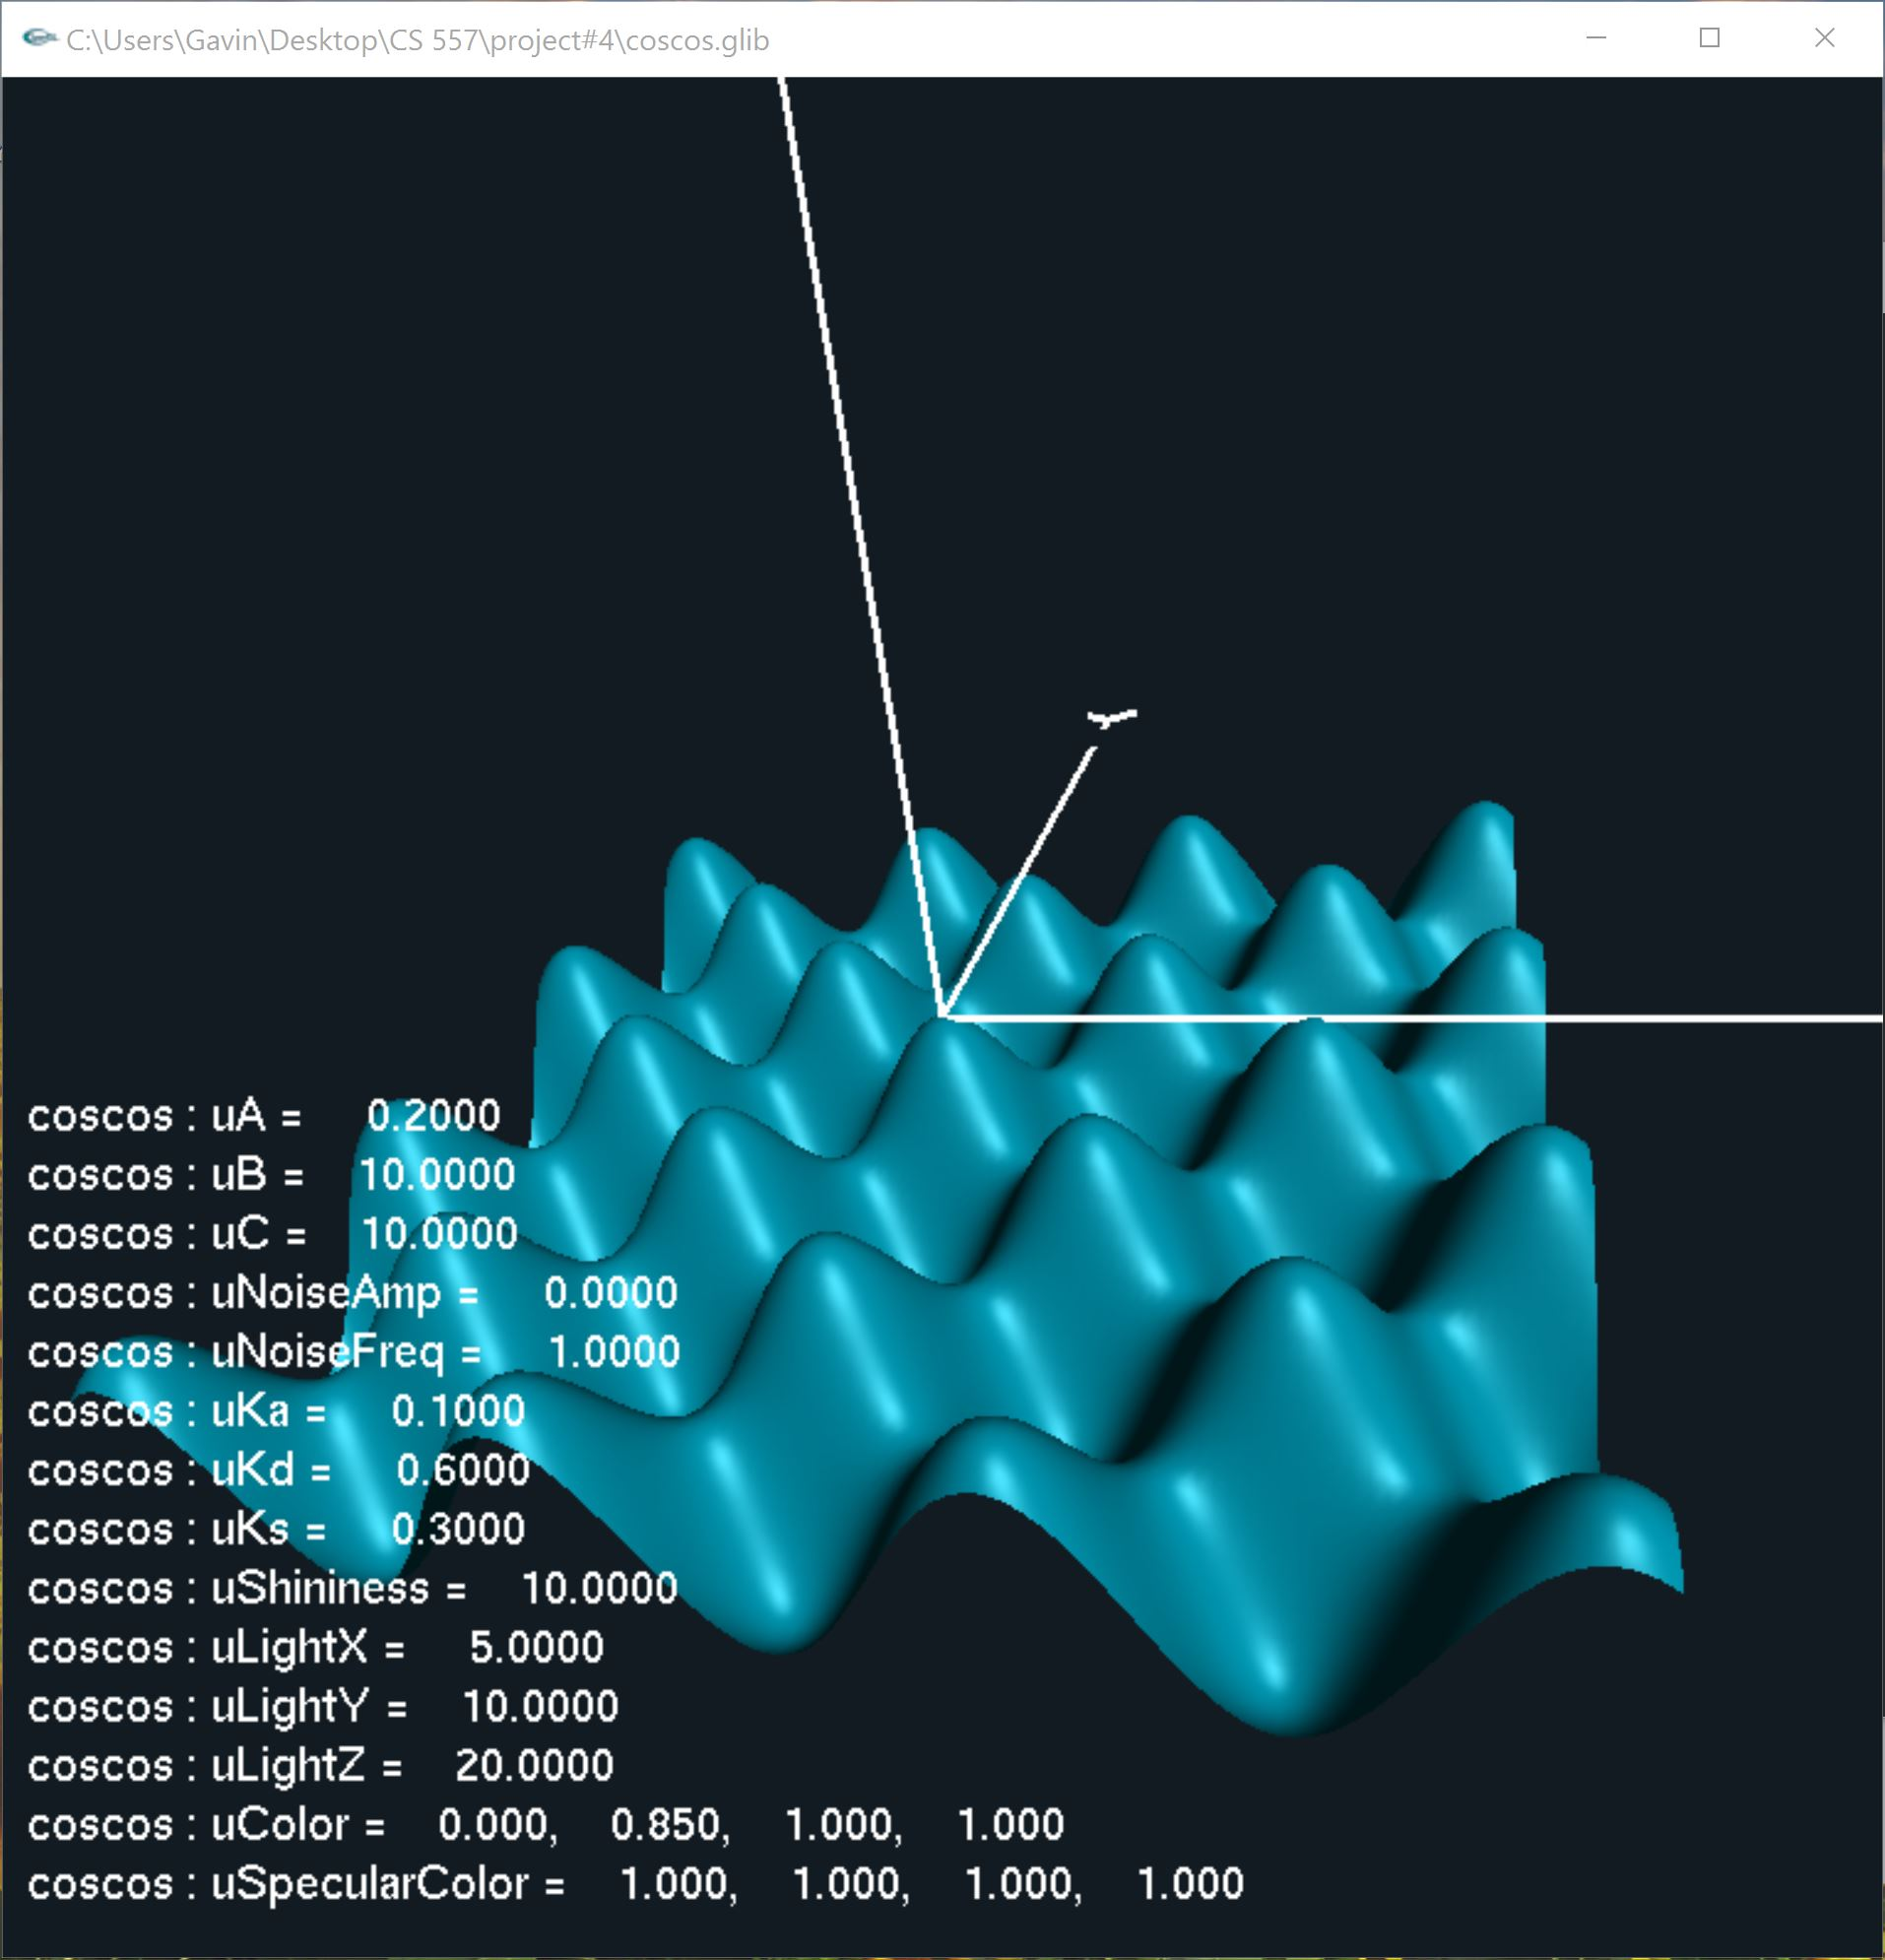
\includegraphics[width=5.5in]{lighting.jpg}
\end{center}
The project has tree sliders named ``uA, uB, uC''. These three sliders control the displacement of the plane. The uA controls the ``height'' fo the displacement. The ``uB'' and ``uC'' controls the number of the ``waves'' in the x and y direction. The ``height'' of the ``waves'' is actually calculated by the equation $Z = uA * cos(uB*x) * cos(uC*y)$, and this is exactly how these three sliders affect the image. The following images show the changes these three sliders make to the plane. The first is changing the ``uA'' slider. The second is changing the ``uB'' slider and the third is changing the ``uC'' slider.
\begin{center}
	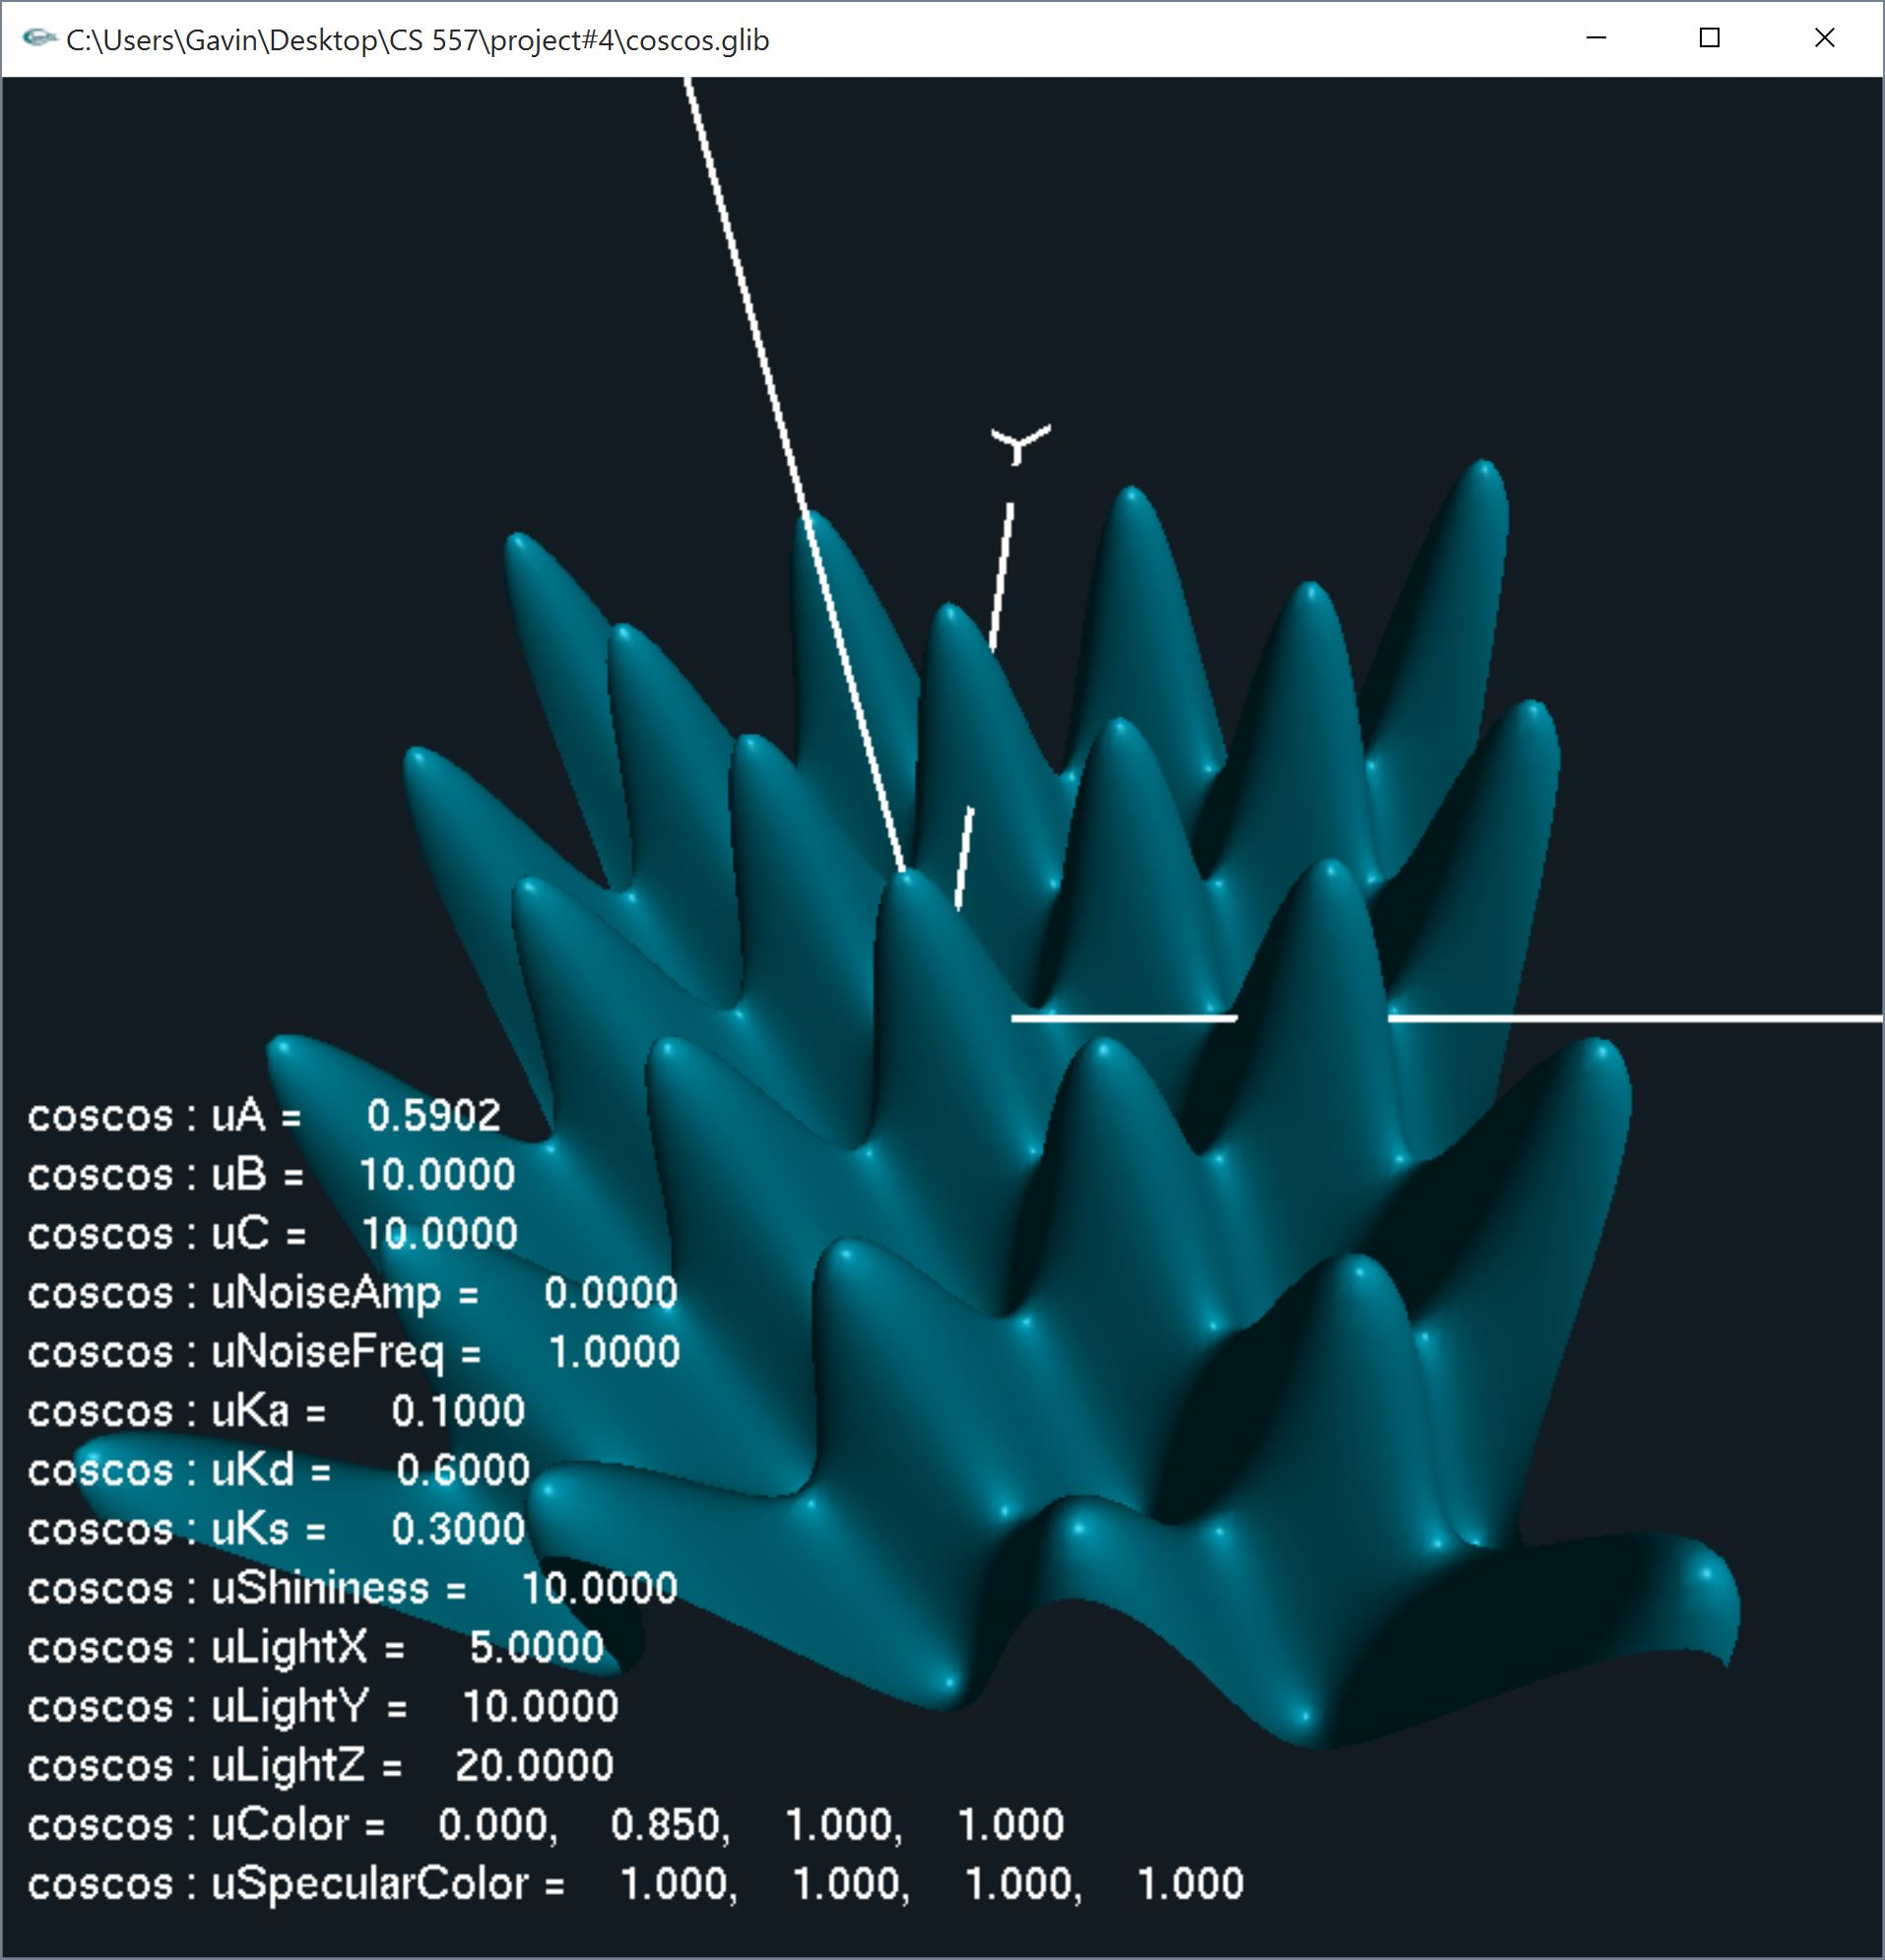
\includegraphics[width=3.2in]{uA.jpg}
\end{center}
\begin{center}
	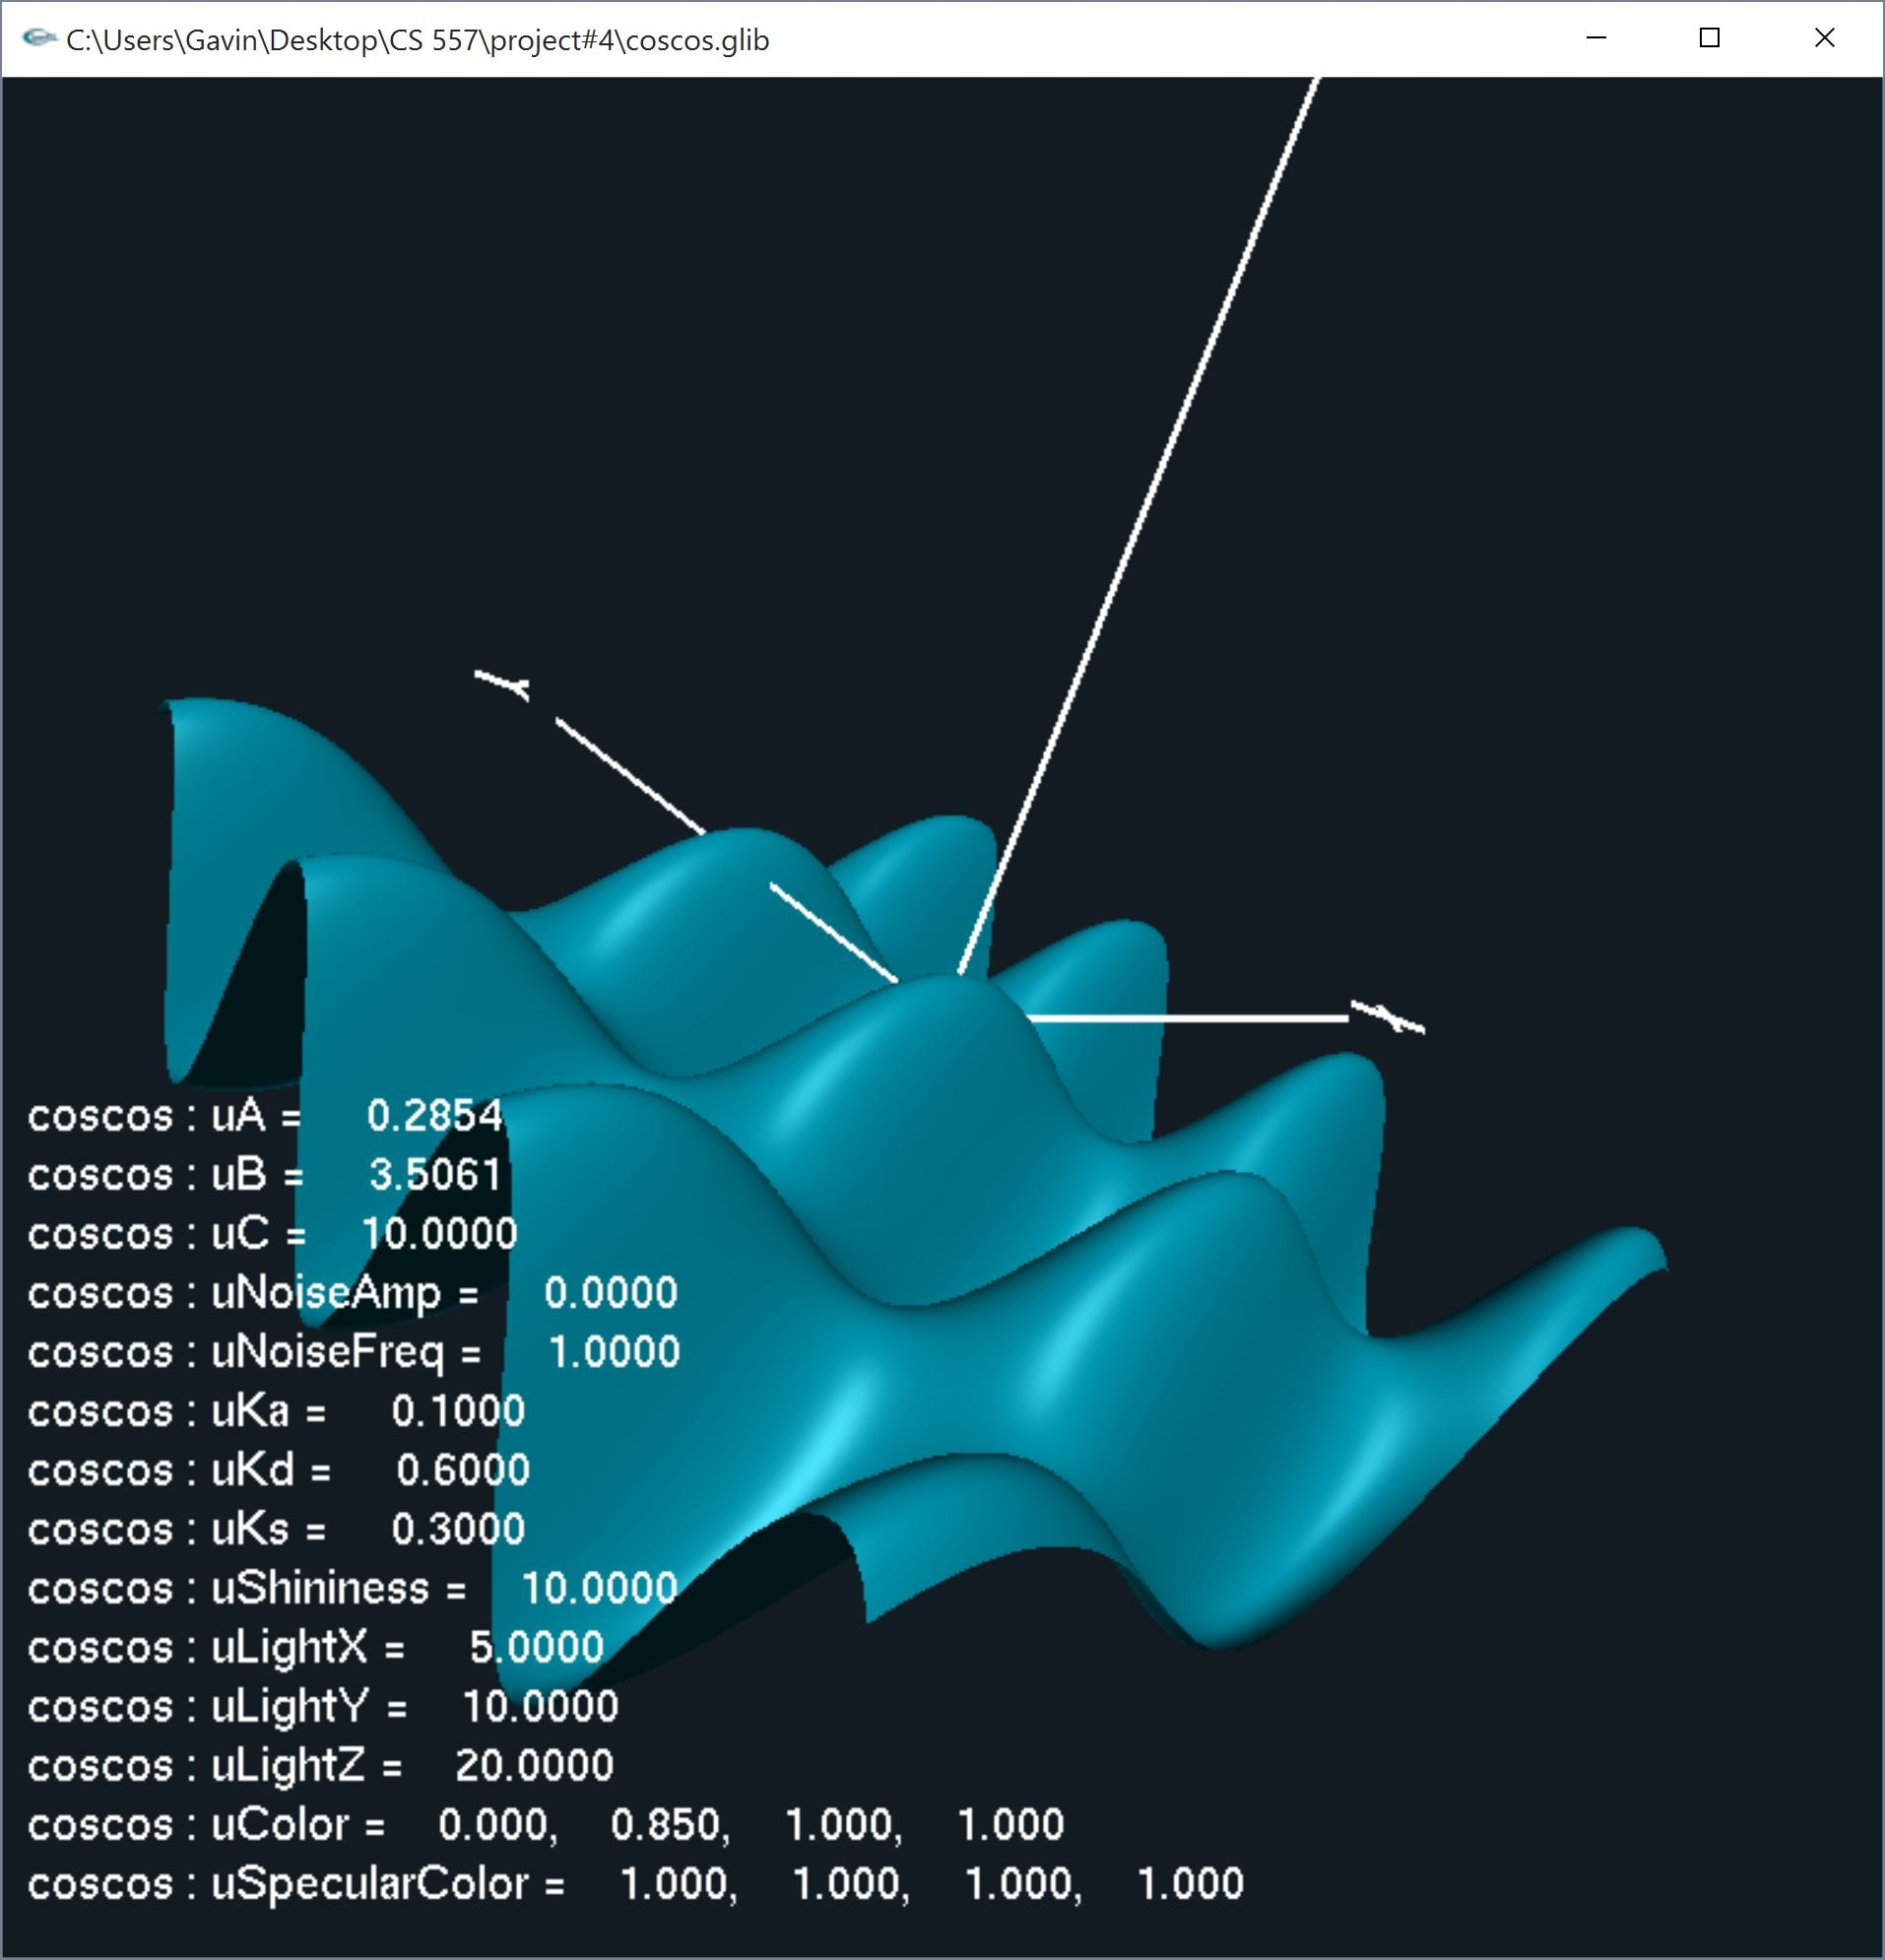
\includegraphics[width=3.2in]{uB.jpg}
	\includegraphics*[width=3.2in]{uC.jpg}
\end{center}
The second part of the project asks us to add noise to the surface using bump mapping. Like the previous project we did, the bump mapping is a fake displacement. It actually changes the normal instead of implement the real displacement. In this project, I did the same thing to the surface. The project has two sliders named ``uNoiseAmp, uNoiseFreq'', which stands for noise amplitude and frequency as previous project. Then the I used these two values to calculate two random angles on x and y direction. By applying these two angles to the fragment's normal, the normal will be rotated to another direction. By using this normal to calculate the lighing, it will result in some ``dark marks'' and ``shiny spots'', which deliver the sense of an irregularity surface but the truth is the surface is still smooth. The following two images show the result of bump mapping from different looking directions. With the fragment lighting, the correctness of bump mapping could be examined.
\begin{center}
	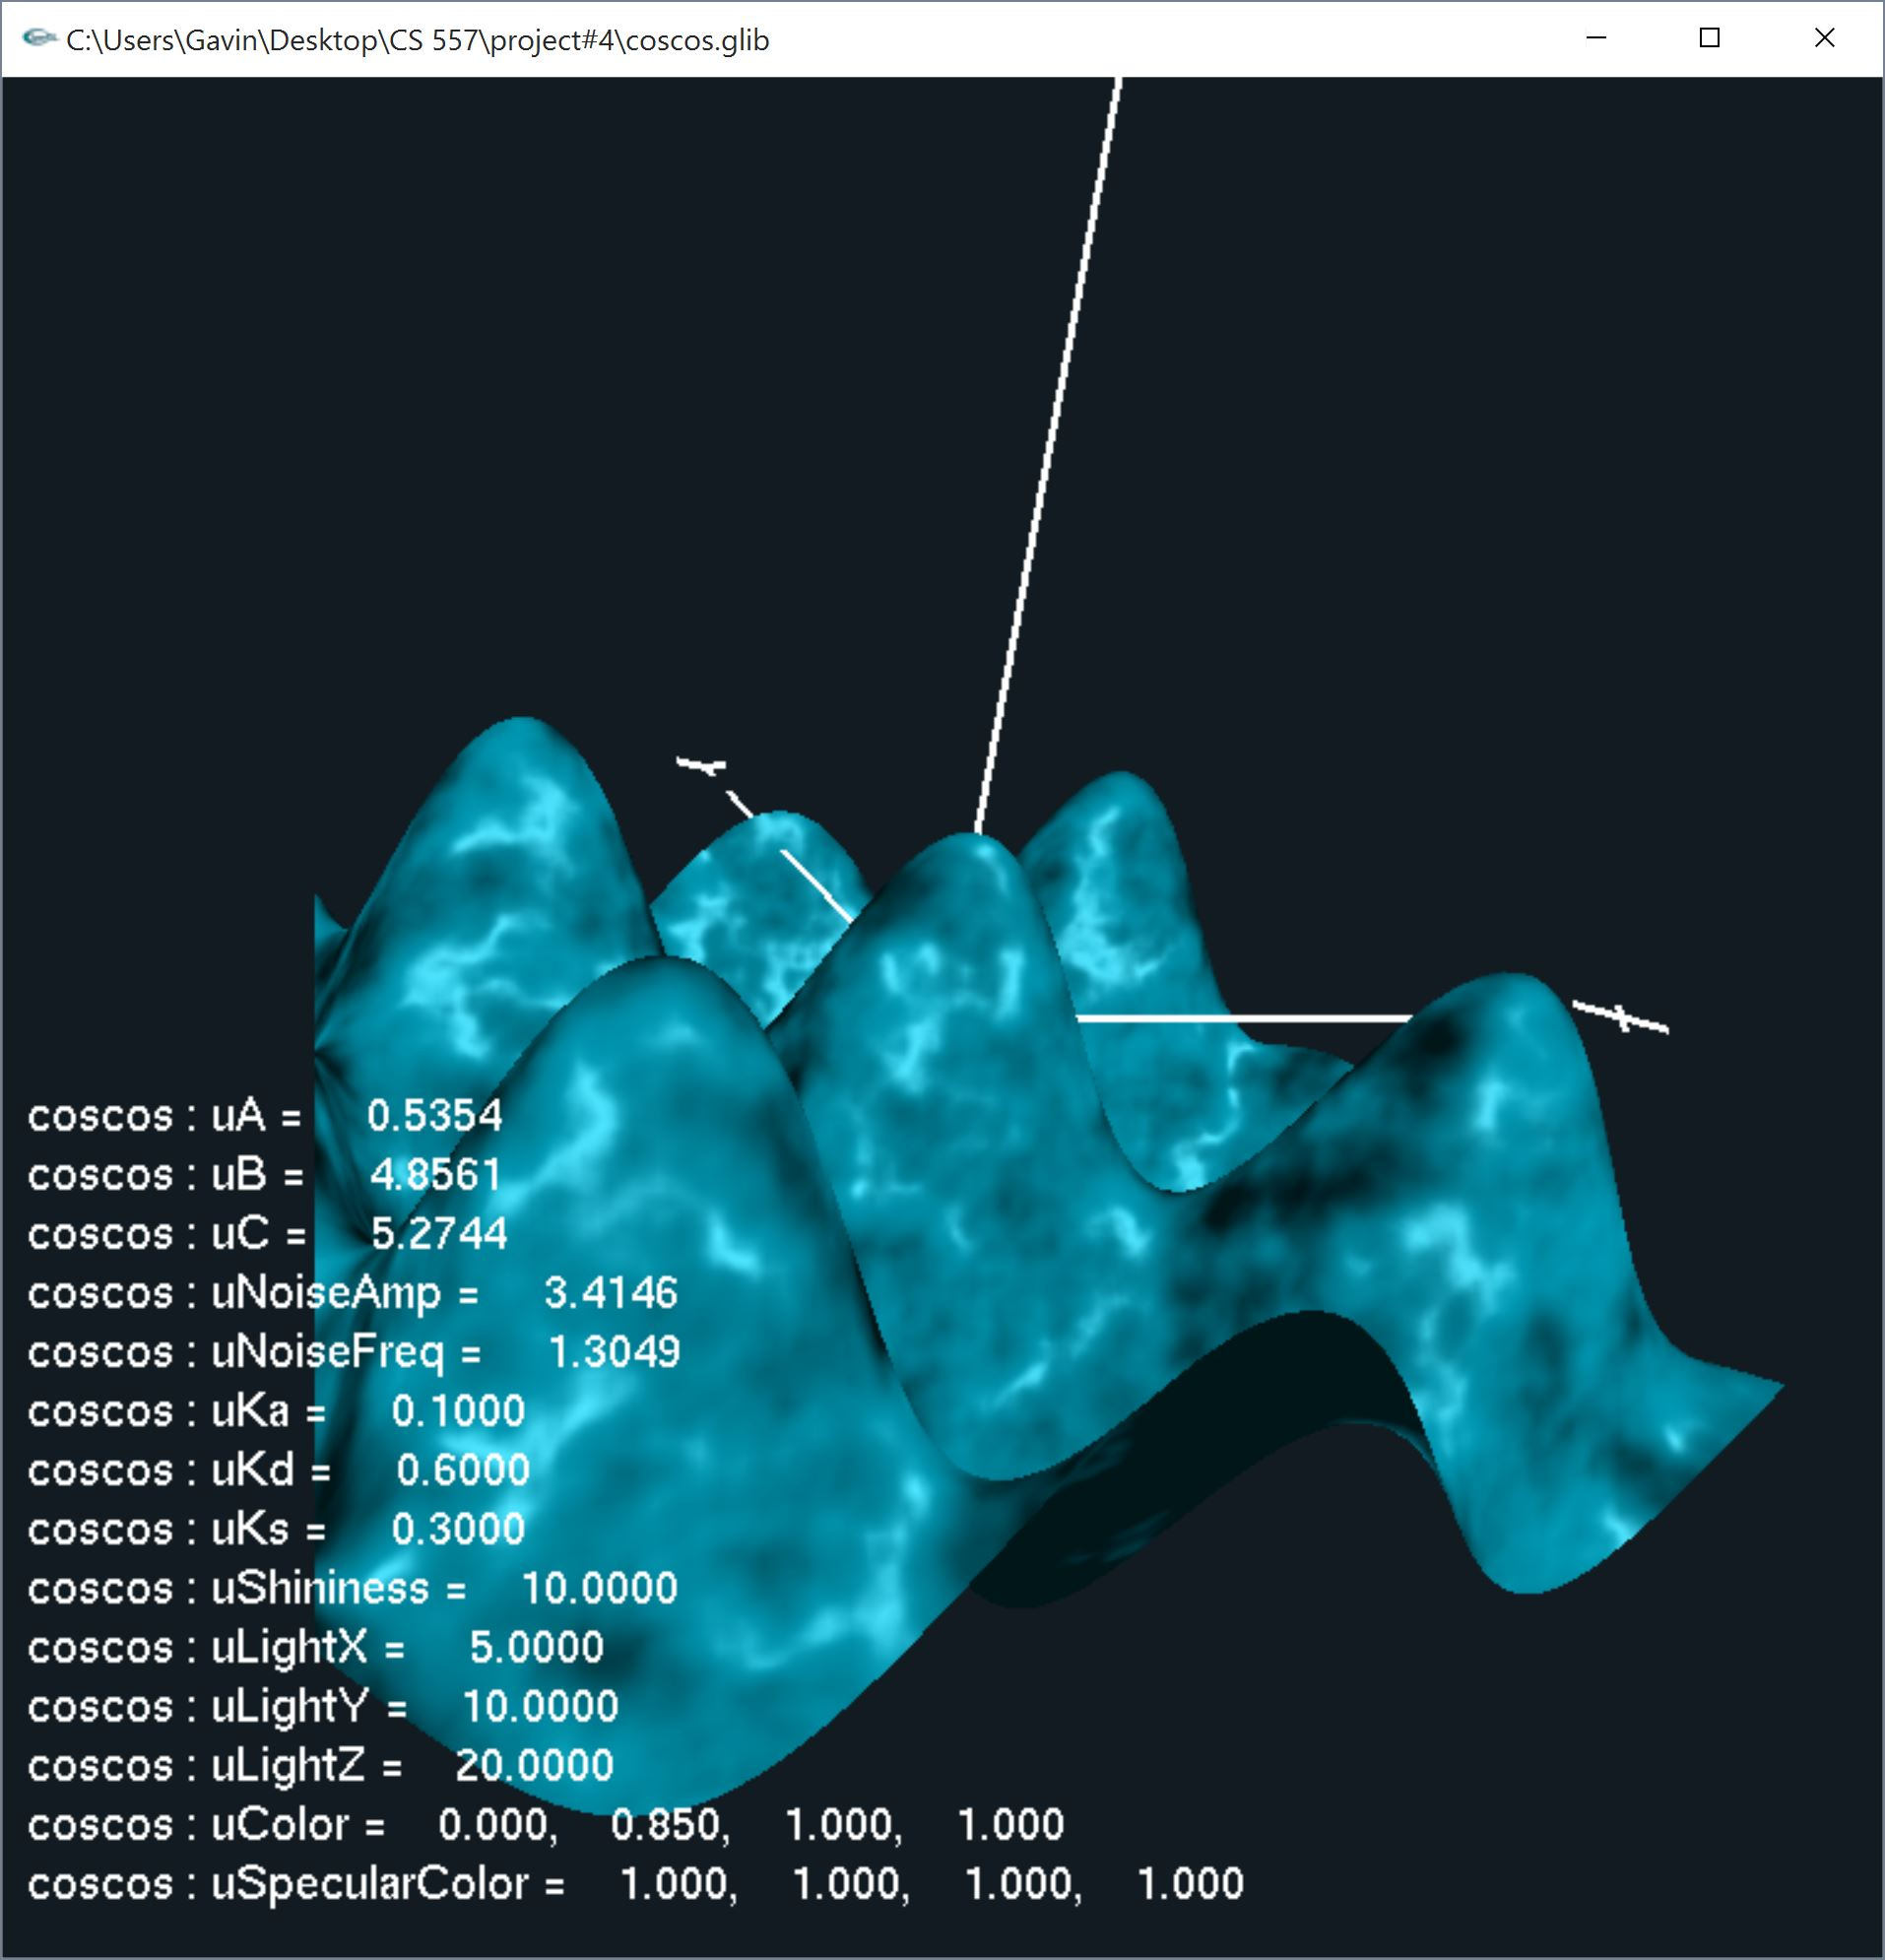
\includegraphics[width=3.2in]{bump1.jpg}
	\includegraphics*[width=3.2in]{bump2.jpg}
\end{center}
The project also has three sliders named ``uLightX, uLightY, uLightZ''. They controls the position of the light. By changing these three sliders, the light source position will be changed. The following image on the left shows the result that the light source position has been changed. The project also has three sliders named ``uKa, uKd, uKs''. These three sliders control the ambient color, diffuse color, and specular color of the light. There also exists one slider named ``uShininess'', which controls the shiny spot on the surface. By changing the four sliders mentioned above, the sense of different materials of the surface will be dilivered. The following image on the right shows the effect that changing these four sliders.
\begin{center}
	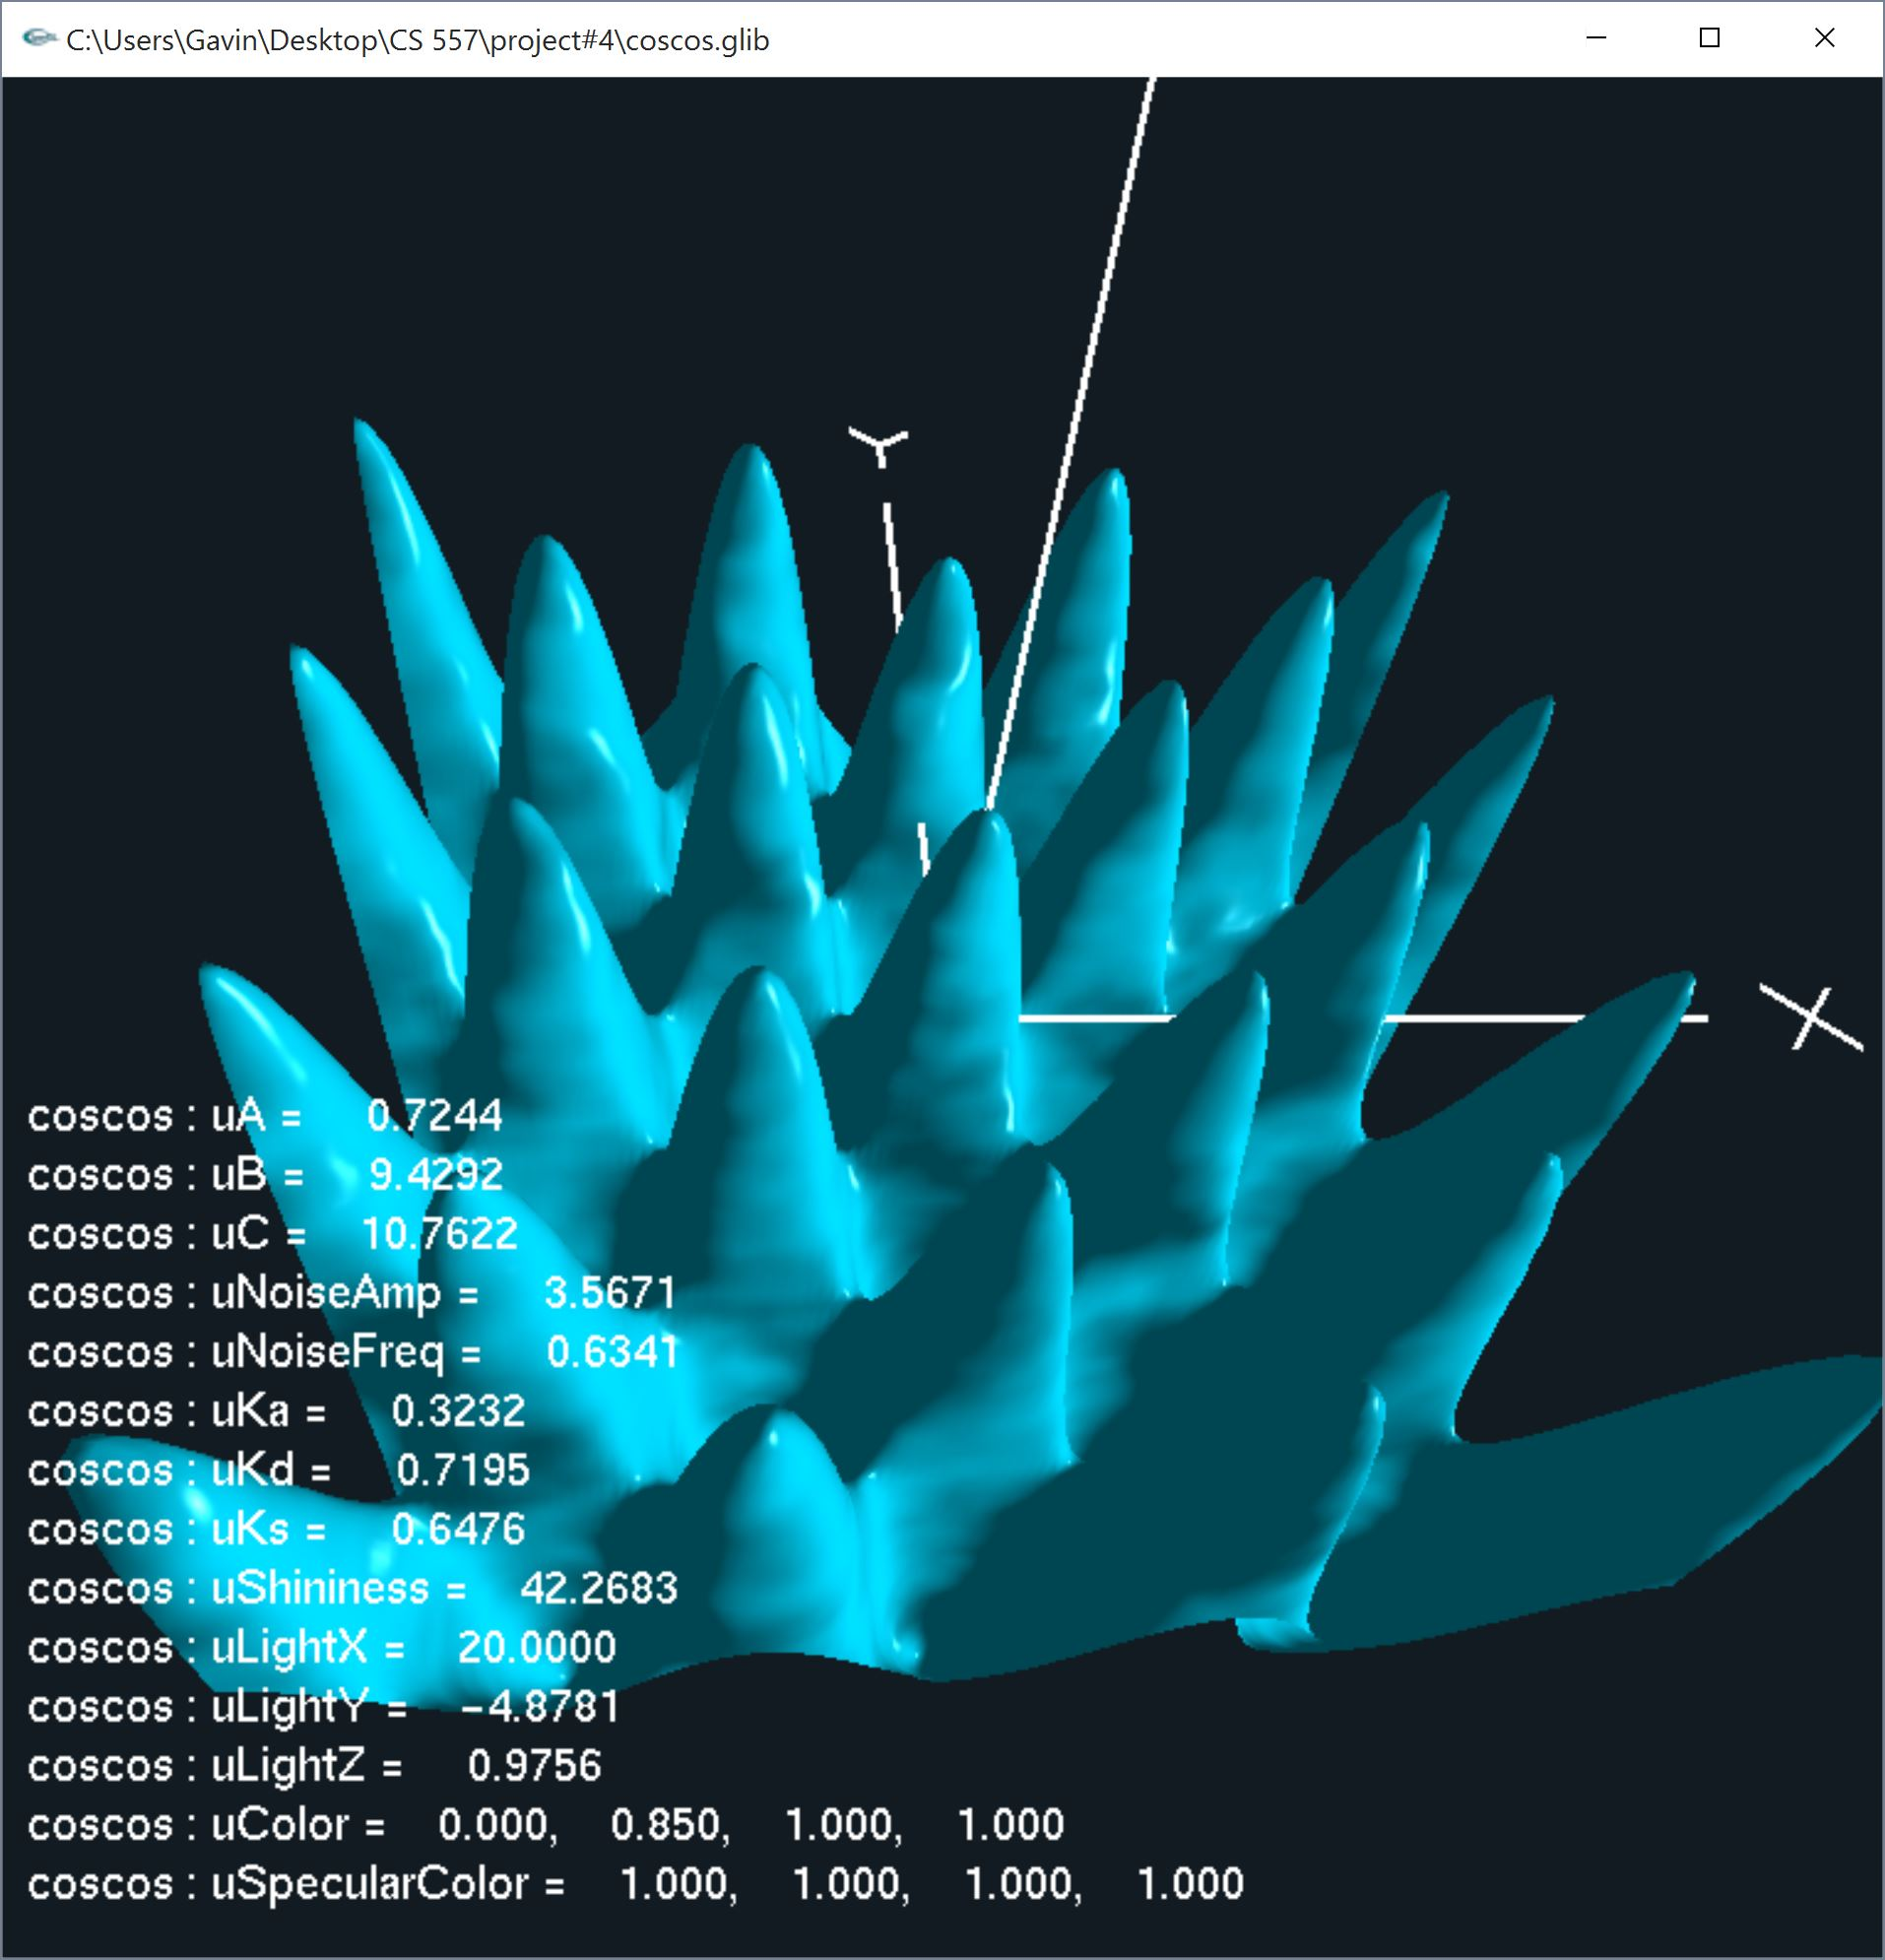
\includegraphics[width=3.2in]{lightxyz.jpg}
	\includegraphics*[width=3.2in]{ads.jpg}
\end{center}

\section{Summary}
This project itself is not hard at all. However, I did get caught by one problem. I timed the noise amplitude to the moise before mapped it to range of $[-1, 1]$, which will result in situation that the whole rotate angle range shifted away. The result image is like the whole surface normal turned around when changing the uNoiseAmp value. Thanks to Prof. Bailey helping me solve the problem so that I could hand in a completed project. Dealing with the problems like this is also fun to me, I would like to do more things about shader and I'm looking forward to the following shader projects and willing to do a lot more on them.
\end{document}